% !TEX encoding = UTF-8
% !TEX TS-program = pdflatex
% !TEX root = ../tesi.tex
% !TEX spellcheck = it-IT

%**************************************************************
\chapter{Introduzione}
\label{cap:introduzione}
%**************************************************************

%Introduzione al contesto applicativo.\\

%\noindent Esempio di utilizzo di un termine nel glossario \\
%\gls{api}. \\

%\noindent Esempio di citazione in linea \\
%\cite{site:agile-manifesto}. \\

%\noindent Esempio di citazione nel pie' di pagina \\
%citazione\footcite{womak:lean-thinking} \\

%**************************************************************
\section{L'azienda}

VIC è stata fondata da Alessio Bisutti che, dopo aver sviluppato una lunga esperienza
nel campo ispettivo, ha deciso di costituire una società in grado di offrire ai propri clienti un servizio professionale, chiaro ed affidabile, appoggiandosi alle nuove tecnologie.
Si occupa di controlli per grandi ordini, sia di materie prime che di semi-lavorati, di
cui individua e riporta eventuali danni, carenze nella spedizione e non conformità con
quanto ordinato.
VIC viene fondata a Venezia 7 anni fa come piccola società di ispezione locale. Fin dall'inizio, l'obiettivo principale di VIC è stato la riduzione del tempo tra ispezione e reporting al cliente. Ora l'obiettivo è raggiunto, perchè VIC sta fornendo ai suoi clienti tutti i risultati e le informazioni importanti in tempo reale, senza alcun ritardo, grazie agli investimenti fatti nel campo della tecnologia e delle applicazioni mobili.

%**************************************************************
\section{L'idea}

I più importanti obbiettivi del controllo qualità effettuato durante un ispezione sono il determinare la corretta forma, peso, quantità e dimensioni degli oggetti da esaminare.\\
Gli ispettori possono scattare fotografie, prendere appunti e sfruttare la loro esperienza per fornire stime accurate; si è manifestata però la necessità di affiancare queste ultime a dei dati quanto più possibile oggettivi e rapidi da ottenere.\\
Da qui nasce l'idea di fornire agli ispettori uno strumento informatico in grado di effettuare queste stime. Grazie alla ricostruzione computerizzata resa disponibile dai \emph{Tango device} sarà possibile non solo visualizzare su uno schermo il modello 3D del soggetto della ispezione, ma anche ottenere ulteriori dati utili quali:
\begin{itemize}
	\item Una stima del volume, e se necessario del peso, dell'oggetto.
	\item L'esito del confronto dell'oggetto con un modello ideale, per evidenziare eventuali danni o deformazioni.
\end{itemize}
Con il prototipo realizzato durante lo \emph{stage} sono rese disponibili solamente le funzionalità di ricostruzione dell'oggetto e calcolo (approssimato) del volume.\\
Le operazioni troppo computazionalmente intensive da effettuare su tablet, quali il filtraggio e \emph{meshing} dei punti acquisiti, sono state delegate ad un \emph{backend server} che effettui le elaborazioni necessarie ed invii i risultati al richiedente, mentre all'applicativo per tablet è stato affidato il compito di aquisire e visualizzare un oggetto sotto forma di 'Nuvola di Punti' e poterne esaminare la \emph{mesh} ottenuta.

%**************************************************************
\section{Cos'è Project Tango}

Project Tango è un \emph{tablet} sperimentale prodotto da \emph{Google} in grado di scandire tridimensionalmente l'ambiente circostante e di tracciare la propria posizione rispetto ad esso. Ciò è possibile attraverso il ricco hardware di cui è dotato (si veda la figura \ref{fig:tango_hardware}), tra cui:
\begin{itemize}
\item una fotocamera RBG-IR\\
\item una fotocamera \emph{Fisheye}\\
\item un sensore di profondità IR\\
\item accelerometro e giroscopio\\
\end{itemize}

\begin{figure}[!h] 
    \centering 
    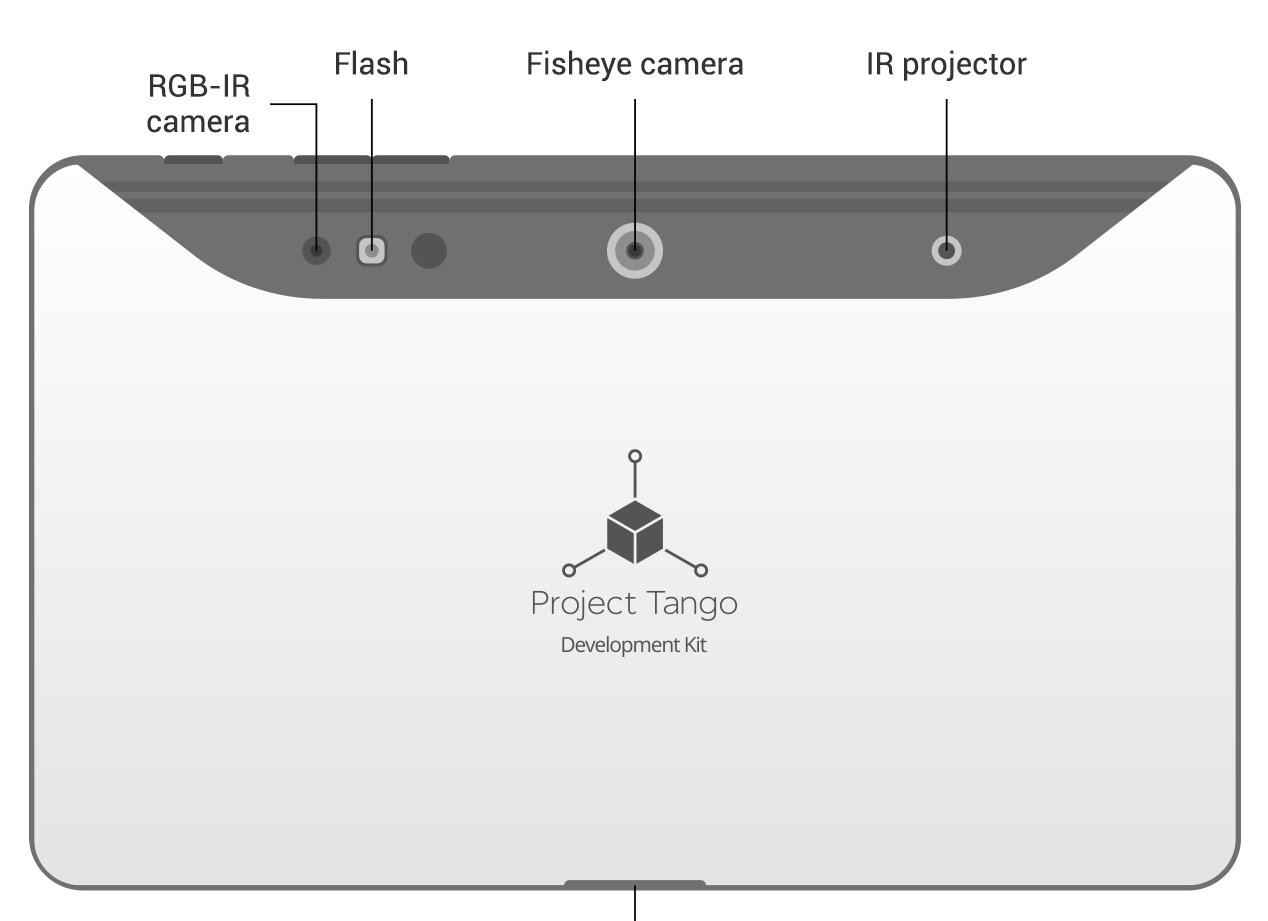
\includegraphics[width=0.9\columnwidth]{varie/tango-hardware.png} 
    \caption{L' \emph{hardware} di \emph{Project Tango}}
    \label{fig:tango_hardware}
\end{figure}

\noindent
Project Tango è quindi specificamente pensato per sviluppare applicazioni che necessitano di comprendere ed estrapolare informazioni dal mondo reale (ad es. realtà aumentata).
Le funzionalità del \emph{tablet} sono accessibili attraverso le \emph{Tango API}, le \emph{API} ufficiali per lo sviluppo di applicazioni \emph{Tango}.


%**************************************************************
\section{Il Prodotto - lato client}

L'applicazione su \emph{tablet} prodotta realizza, seppur non in maniera completa, le esigenze citate al punto precedente. \\
La sua realizzazione ha incontrato molte problematiche talvolta critiche e difficili da prevedere. Per questo durante lo sviluppo sono stati implementati più prototipi, al fine di esplorare le potenzialità e soprattutto i limiti del \emph{tablet} e delle \emph{Tango API}. \\
Lo scopo principale dell'applicazione lato \emph{tablet} è quello di rilevare una corretta 'Nuvola di Punti' dell'oggetto che si vuole esaminare.\\
Una 'Nuvola di Punti' è una descrizione matematica di un oggetto tridimensionale ottenuta tramite un insieme, il più possibile fitto, di punti che lo compongono, definiti dalle loro coordinate (\textbf{x},\textbf{y},\textbf{z}) rispetto ad un fissato sistema di riferimento. \\
Tale rappresentazione, riferita spesso d'ora in poi con il più elegante termine inglese \emph{Point Cloud}, è facilmente comprensibile all'utente se visualizzata come in figura \ref{fig:point_cloud_example}.
\begin{figure}[!h] 
    \centering 
    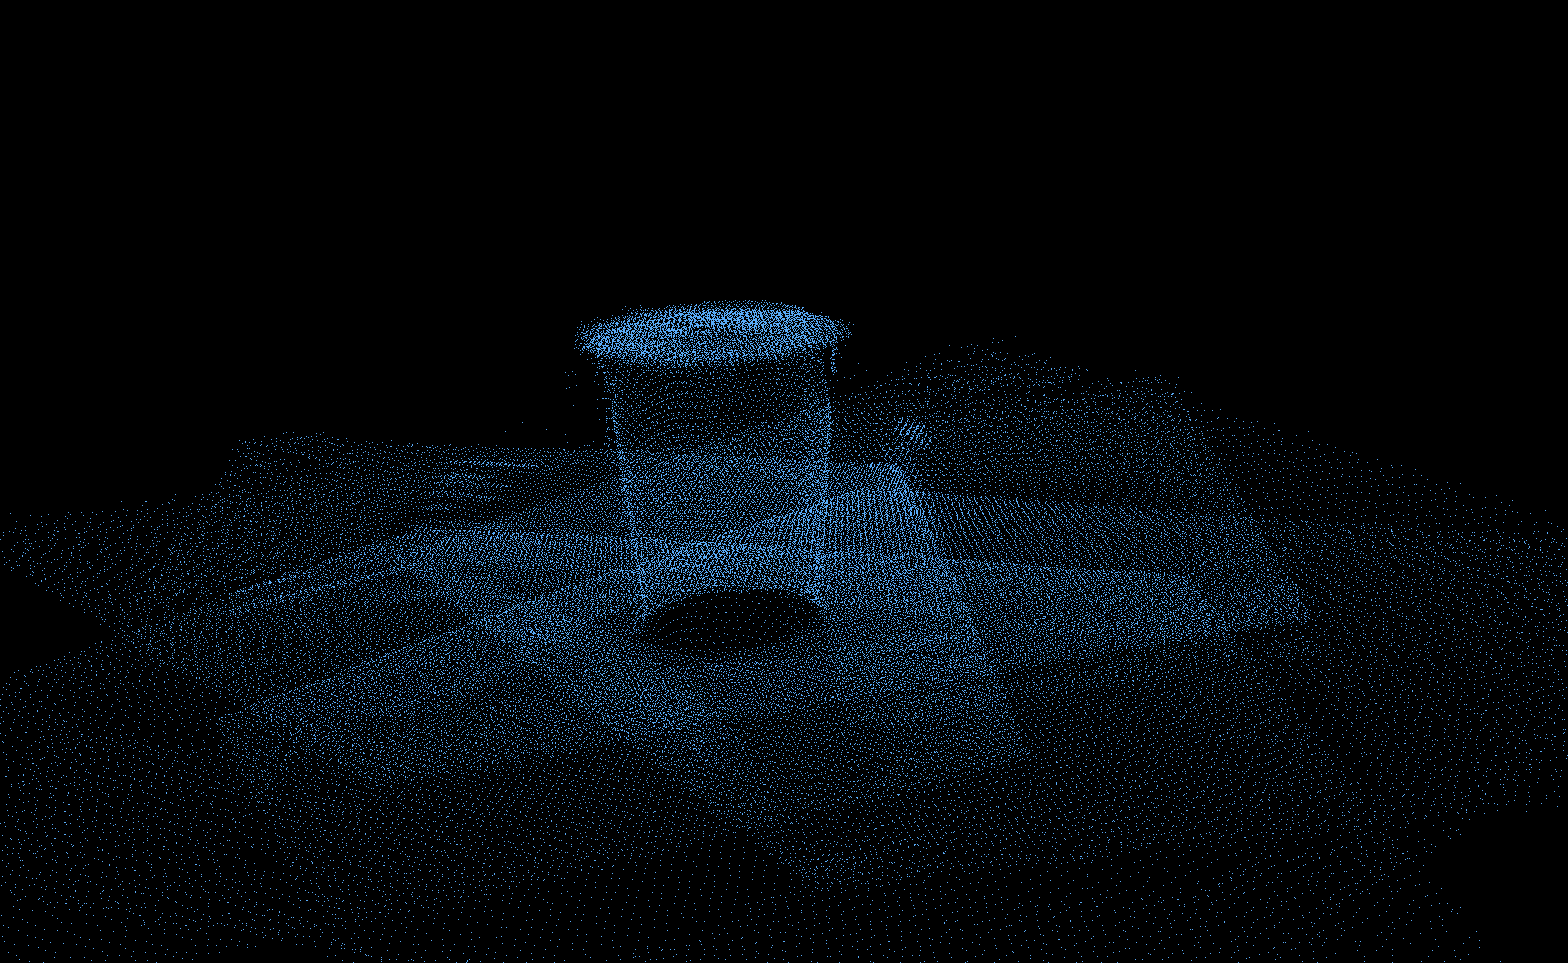
\includegraphics[width=1.0\columnwidth]{varie/point_cloud_example.png} 
    \caption{Esempio di \emph{Point Cloud}: un cestino cilindrico}
   \label{fig:point_cloud_example}
\end{figure}

\subsection{Primo prototipo: Cloude}
Il prototipo denominato \emph{Cloude} risponde all'esigenza di catturare più \emph{Point Cloud} da più angolazioni in modo da ricostruire l'oggetto scansionato sovrapponendo i dati acquisiti. \emph{Cloude} è il risultato di più prototipazioni precedenti effettuate dallo stagista che ha iniziato il progetto prima di me e con cui ho strettamente collaborato.\\
Il prototipo permette quindi di acquisire più \emph{Point Cloud} in successione, ognuno dei quali verrà adeguatamente ruotato e traslato rispetto allo spostamento del \emph{tablet}, in modo che la sovrapposizione degli stessi vada infine a ricostruire tutte le parti dell'oggetto esaminato.\\
Una sola acquisizione da una certa angolazione non può infatti comprendere un oggetto nella sua interezza, come dimostrato nelle figure //TODO
 è necessario ricostruire passo per passo un unico \emph{Point Cloud} rappresentante l'oggetto completo.
Sulla base dei risultati di \emph{Cloude} ho iniziato il mio lavoro sulla parte di elaborazione lato \emph{server} dei \emph{Point Cloud} acquisiti; questo è stato inoltre il punto di inizio per lo sviluppo dei prototipi successivi in collaborazione con l'altro stagista.

\subsection{Secondo prototipo: Samba}
Il secondo prototipo parte dai risultati ottenuti con \emph{Cloude} e ne migliora prestazioni e precisione, aggiungendo alcune funzionalità utili. \\
\emph{Samba} affronta e risolve alcuni problemi del prototipo precedente, come il \emph{"Drifting"} e alcuni problemi prestazionali dovuta alla mole elevata di dati acquisiti. Introduce inoltre la funzionalità di visualizzazione delle \emph{mesh} elaborate dal \emph{server}.

\subsubsection{Drift correction}
Il prototipo precedente, seppur funzionale, generava ricostruzioni di scarsa qualità, afflitte soprattutto dal problema del \emph{"drifting"}. Il \emph{drifting} è un problema comune nelle applicazioni di realtà aumentata, che come \emph{Project Tango} usano la tecnica del \emph{Motion Tracking}, cioè aggiornano costantemente la propria posizione relativamente alle coordinate acquisite nella posizione precedente, mantenendo così una storia dei movimenti del \emph{device} rispetto all'ambiente circostante.\\
Ad ogni aggiornamento della posizione è normale ed inevitabile che la misurazione, per quanto precisa, introduca un piccolo errore; la catena di errori sommati porta quindi col passare del tempo ad un'importante discrepanza tra la posizione stimata del \emph{device} e la sua posizione reale, come evidenziato in figura \ref{fig:drift_correction}
\begin{figure}[!h] 
    \centering 
    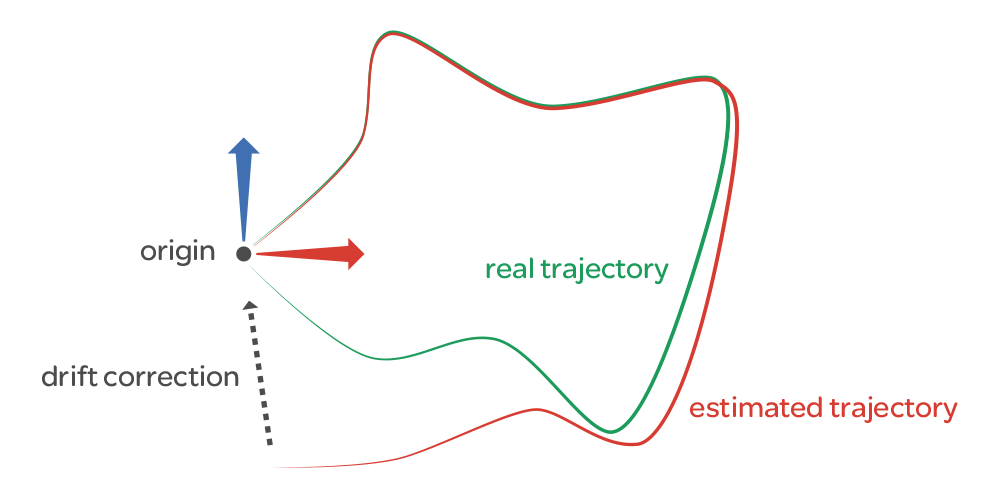
\includegraphics[width=0.9\columnwidth]{varie/Drift_Correction.png} 
    \caption{\emph{Drifting} nel \emph{Motion Tracking}}
    \label{fig:drift_correction}
\end{figure}
Per ovviare in parte a questo problema \emph{Samba} utilizza una tecnica chiamata \emph{Drift Correction} ch si appoggia sulle funzionalità di \emph{Area Learning} dei \emph{device Tango}.\\
L' \emph{Area Learning} consiste nella capacita del dispositivo di estrarre dallo spazio fisico che sta analizzando una serie di punti significativi (o \emph{key features}), facilmente riconoscibili, e di salvare tali informazioni per confrontarle con le successive acquisizioni. In questo modo il dispositivo è capace di riconoscere un'area precedentemente visitata, e può quindi applicare le necessarie correzioni alla popria stima della traiettoria, di qui il nome \emph{Drift Correction}.\\
Con l'implementazione di questa funzionalità è necessario, prima di iniziare la ricostruzione di un \emph{Point Cloud}, riprendere l'oggetto e i suoi dintorni per un po' di tempo e da diverse angolazioni, in modo da permettere al \emph{tablet Tango} di costruire una mappa, detta \emph{Area description}, dell'area circostante, e di stabilizzare la traiettoria stimata con le informazioni acquisite.\\
I risultati si vedono confrontando queste due ricostruzioni di una scatola, vista dall'alto (fig. \ref{fig:no_drift_correction} e fig. \ref{fig:with_drift_correction}), rispettivamente senza e con \emph{Drift correction}.
\begin{figure}[htp] 
    \centering
    \subfloat[Ricostruzione senza \emph{Drift correction}]{%
        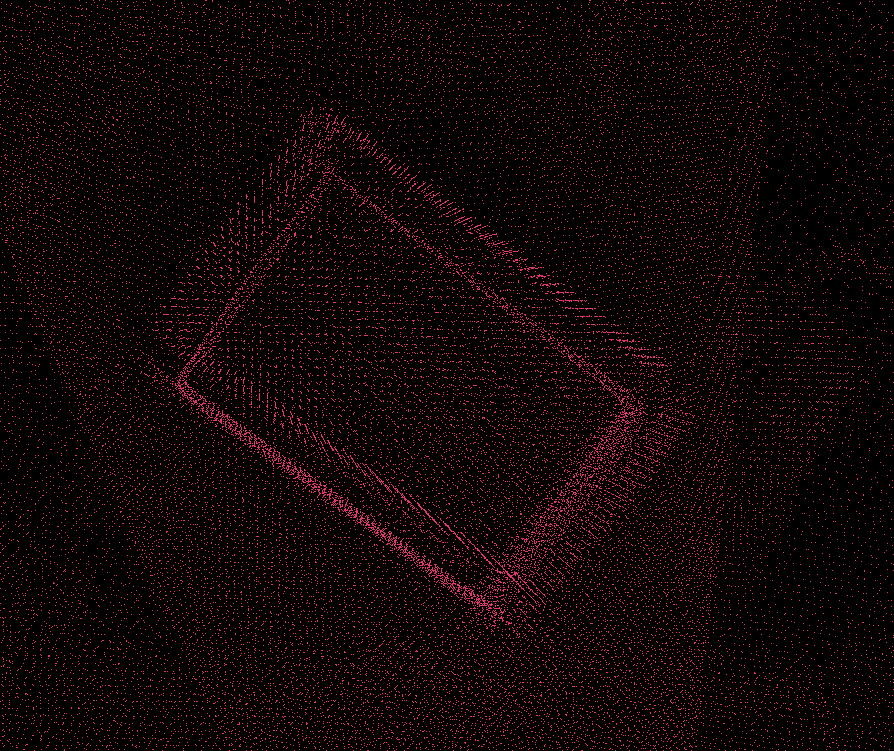
\includegraphics[width=0.47\columnwidth]{varie/no_drift_correction.png} 
    	%\caption{Ricostruzione senza \emph{Drift correction}}
    	\label{fig:no_drift_correction}
    }%
    \hfill%
    \subfloat[Ricostruzione con \emph{Drift correction}]{%
        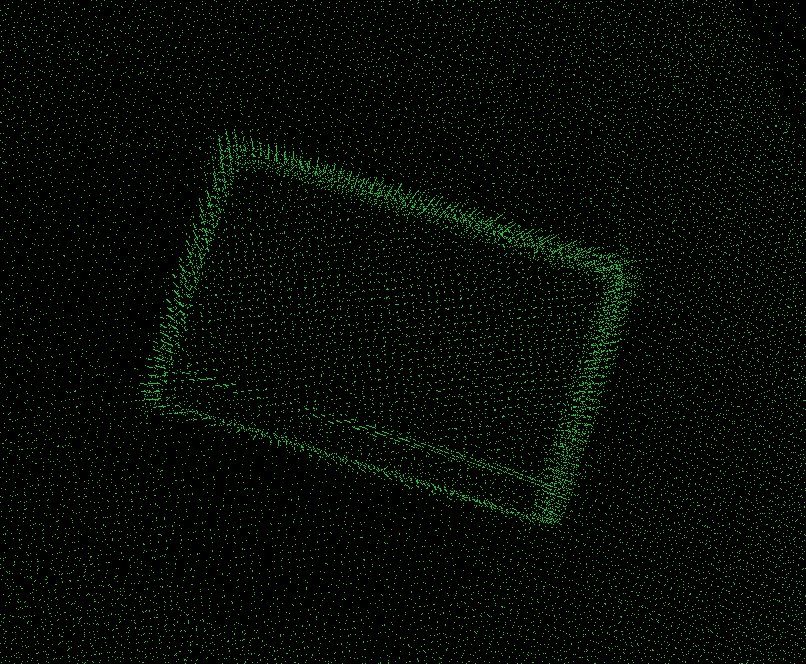
\includegraphics[width=0.47\columnwidth]{varie/with_drift_correction.png} 
    	%\caption{Ricostruzione con \emph{Drift correction}}
    	\label{fig:with_drift_correction}
    }%
    \caption{Benefici della \emph{Drift Correction}}
\end{figure}
\newline
Come si nota in figura \ref{fig:with_drift_correction} il risultato non è ancora ottimale, infatti un lato della scatola appare sdoppiato e spostato di qualche centimetro; si tratta di un problema di \emph{ghosting} di cui verrà trattato più avanti.

\subsubsection{Prestazioni}
Il prototipo precedente presentava due problemi prestazionali principali:
\begin{itemize}
\item La ricostruzione passo per passo del \emph{Point Cloud} finale era troppo lenta
\item La mole dei dati trattati al sovrapporsi di più \emph{Point Cloud} diventava proibitiva
\end{itemize}
\noindent
Il primo problema si presentava utilizzando i metodi forniti dalla libreria \emph{Tango} per trasformare le coordinate relative dei punti in coordinate assolute per permetterne la giusta sovrapposizione. Tale metodo, seppur di facile utilizzo, diventava troppo dispendioso all'aumentare delle dimensioni del \emph{Point Cloud}, che raggiunge facilmente gli 80.000 punti.\\
Per risolvere il problema viene quindi creata, per ogni \emph{Point Cloud}, una \emph{matrice di rototraslazione} che rappresenta lo spostamento e la rotazione del dispositivo rispetto al sistema di riferimento, e viene moltiplicato il vettore delle coordinate di ogni singolo punto per la matrice generata. \\
In questo modo si sono ridotti i tempi di elaborazione dell'80\%;

\noindent
Il secondo problema era causato dal sovrapporsi di molti punti quasi identici, ad esempio i punti rappresentanti il pavimento. Partendo dall'osservazione che una certa quantità di punti molto vicini può essere trasformata in un unico punto, valore medio di tutti gli altri, senza una significativa perdita d'informazione, \emph{Samba} risolve il problema attraverso una tecnica di \emph{voxeling}.\\
Lo spazio viene suddiviso in tanti piccoli parallelepipedi (tipicamente cubi) di uguali dimensioni; tutti i punti che ricadono all'interno di un singolo parallelepipedo, o \emph{voxel}, vengono considerati come un unico punto. Così facendo si riducono sensibilmente le dimensioni del \emph{Point Cloud} senza alterarne negativamente la precisione.
Di seguito la differenza visivamente evidente tra lo stesso Point Cloud filtrato prima con voxel cubici di lato 1cm (fig. \ref{fig:low_voxeling}) e poi di lato 3cm (fig. \ref{fig:high_voxeling}), con una differenza di circa 60.000 punti rimossi in più nella seconda elaborazione.
\begin{figure}[htp] 
    \centering
    \subfloat[Voxeling leggero]{%
        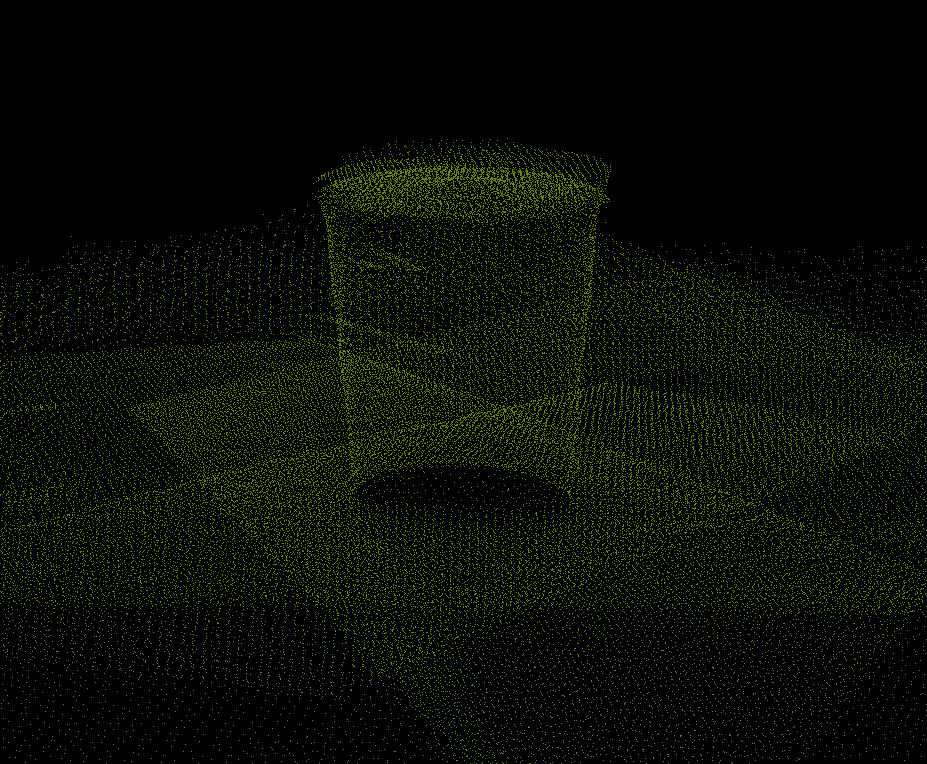
\includegraphics[width=0.47\columnwidth]{varie/low_voxeling.png} 
    	\label{fig:low_voxeling}
    }%
    \hfill%
    \subfloat[Voxeling elevato]{%
        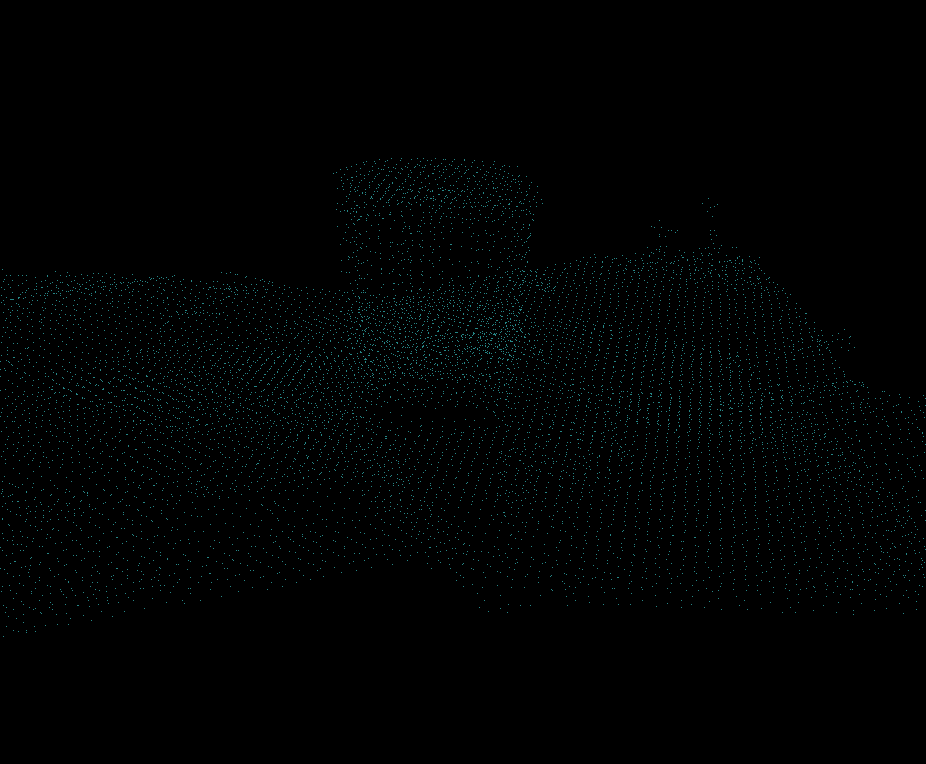
\includegraphics[width=0.47\columnwidth]{varie/high_voxeling.png} 
    	\label{fig:high_voxeling}
    }%
    \caption{Effetti del \emph{voxeling}}
\end{figure}
\newline

\subsubsection{Visualizzatore di mesh}
Nel prototipo è stata introdotta la possibilità di caricare e visualizzare le \emph{mesh} risultato dell'elaborazione lato server di un \emph{Point Cloud}.
Una \emph{mesh} poligonale è una collezione di vertici, spigoli e facce che definiscono la forma di un oggetto poliedrico; in \emph{Samba} è ottenuta a partire dalla nuvola di punti elaborata.
Tale \emph{mesh} viene salvata dal \emph{server} in formato \emph{OBJ}, comunemente usato nelle applicazioni 3D. Dall'applicazione viene quindi richiesto di caricare e salvare nella memoria locale del tablet le mesh disponibili sul server, per poi poter essere visualizzate ed esaminate.


\subsection{L'applicativo attuale: VIC-Tango}

\subsubsection{Firebase}
\subsubsection{JNI}
\subsubsection{Camera preview}
%\subsection{Bug fixing}

%**************************************************************
\section{Il Prodotto - lato server}



%**************************************************************
\section{Organizzazione del testo}
Riguardo la stesura del testo, relativamente al documento sono state adottate le seguenti convenzioni tipografiche:
\begin{itemize}
	\item gli acronimi, le abbreviazioni e i termini ambigui o di uso non comune menzionati vengono definiti nel glossario, situato alla fine del presente documento;
	\item per la prima occorrenza dei termini riportati nel glossario viene utilizzata la seguente nomenclatura: \emph{parola}\glsfirstoccur;
	\item i termini in lingua straniera o facenti parti del gergo tecnico sono evidenziati con il carattere \emph{corsivo}.
\end{itemize}